\section[Rendering]{Rendering\cite{GLReference, OglDev, ThinMatrix, SparkyEngine, GLTut}}
\label{rendering}
\subsection{OpenGL Grundlagen}

Die FM3D-Engine verwendet für die Darstellung von dreidimensionalen Szenen die Grafikbibliothek OpenGL. Mit OpenGL ist es möglich verschiedene kleine grafische Objekte zu rendern. Dieses entsprechen drei geometrischen Grundobjekte (\textit{Primitives}): 
Punkte, Linien und Dreiecke. Zudem gibt es verschiedene Möglichkeiten diese aneinander zu reihen, wie in \cref{OpenGLPrimitives} dargestellt ist. Sie können alle einzeln, aber auch aneinanderhängend gerendert werden. Bei letzteren kann Speicher bei den angrenzenden Eckpunkten gespart werden. Diese \textit{Primitives} werden durch ihre Eckpunkte oder auch \textit{Vertices} genannt definiert. 
Sie beschreiben eine Position in einem dreidimensionalen Raum. OpenGL arbeitet mit einem orthografischem Koordinatensystem. Das heißt: alle drei Achsen sind orthogonal zueinander und reichen von den Werten -1 bis 1.

\subsubsection{Frame-Buffer}
Das aktuelle Bild wird in mehreren Buffern gespeichert. Die Größe der Buffer ist direkt proportional zu der Pixelanzahl des \textit{Viewports}, also zu dem Bereich, in welchem das gerenderte Bild dargestellt wird. 
Am relevantesten ist der Color-Buffer, der die Farbe jedes Pixels in vier Floats speichert. Jeweils einen für Rot, Grün, Blau und einen Alpha-Wert, welcher die Transparenz beschreibt. Des Weiteren gibt es den Depth-Buffer. Dieser ist selten auch als Z-Buffer in der Literatur zu finden. Er beschreibt den Abstand zwischen dem aktuell gerenderten Pixel und der Kameraebene. Diese Information wird als Farbinformation in dem Depth-Buffer gespeichert. 
\todo[inline]{Channels? Wird nie erwähnt}
Man benötigt nur einen Channel, da nur ein einziger Zahlenwert gespeichert werden muss. So ist, wenn man den Buffer anzeigt, nur ein Schwarz-Weiß-Bild zu sehen. 
Je heller der Pixel ist, desto weiter weg befindet er sich. Die Größe des Depth-Buffer ist einstellbar. Je größer er ist, desto größer ist auch die Präzision, wobei der Depth-Buffer immer eine viel größere Präzision in der Nähe der Kamera besitzt und nach weiter hinten an Präzision verliert. Dies ist von Vorteil, wenn Objekte sehr nah an der Kamera gerendert werden, da dort eine sehr hohe Präzision erforderlich ist. 
Die Präzision ist aber nicht sehr relevant, wenn das Objekt weiter entfernt ist. Der Depth-Buffer ist optional. Wird er nicht verwendet, so kann die räumliche Anordnung der Primitives nicht ermittelt werden. Welcher Pixel am Ende angezeigt wird, ist von der Reihenfolge, in der die Primitives gerendert werden, abhängig. Wobei das zuletzt gerenderte Primitive ganz vorne zu sehen ist. Diese Buffer sind in \cref{DepthBuffer} dargestellt. 

Zudem gibt es noch den \textit{Stencil-Buffer}. Dieser ist ebenfalls optional und ordnet jedem Pixel einen bestimmten Wert zu. Er kann verwendet werden, um bei bestimmten Pixeln das Rendern zu verhindern. Wie er dies umsetzt, ist einstellbar. Es ist möglich verschiedene Operationen durchzuführen, wenn ein Pixel gerendert wird. Es ist zum Beispiel möglich, dass der Stencil-Wert auf 1 gesetzt oder um 1 erhöht wird. 
Zudem ist es möglich den Stencil-Test einzustellen. Dieser wird bei jedem Renderprozess eines Pixels ausgeführt. So kann man zum Beispiel erreichen, dass nur dort, wo der Stencil-Buffer den Wert 1 besitzt, ein Pixel gerendert wird. 
\todo[inline]{folgender Satz ganz komisch. Entweder überarbeiten oder mir zum umschreiben erläutern. Gruß Max :)}
Dadurch können \textit{Schablonen} erstellt werden, bei welchen Objekte gerendert und bei welchen nicht gerendert werden können, daher auch der Name.

Alle Buffer zusammen werden in einem \ac{FBO} gespeichert. Dieses ermöglicht das gleichzeitige Aktivieren aller zugehörigen Buffer, sowie das Anzeigen des Color-Buffers auf dem Bildschirm. Es muss nicht speziell ein \ac{FBO} erstellt werden. Wenn keines erstellt wird, so wird standardmäßig direkt auf den \textit{Screen-Buffer} gerendert. Ein weiterer Vorteil ist, dass man ein \ac{FBO} sowohl als Output (dies ist die häufigere Verwendung) aber auch auch als Input verwenden kann. So kann man zum Beispiel eine gerenderte 3D-Szene in einer anderen 3D- oder 2D-Szene einfügen.  

\subsubsection{Buffer Objects}
Will man einen oder mehrere dieser \textit{Primitives} rendern, so laufen die Daten, welche diese \textit{Primitives} definieren, durch verschiedene Schritte. Diese werden in der Literatur auch oft als die "`Rendering-Pipeline"' bezeichnet. Bei Verwendung dieser Pipeline können immer nur eine Art von Primitives gleichzeitig gerendert werden.
Die Daten werden dabei als Buffer auf der \ac{GPU} gespeichert. Verwendet werden dazu die \acp{VBO}, welche als Byte-Arrays vorliegen. Bei ihnen muss manuell eingestellt werden, wie diese Bytes interpretiert werden sollen. Dafür beschreibt man verschiedene Attribute mit Byte-Anzahl und Größe sowie DatenTyp. Zum Beispiel beschreiben die ersten 4 Bytes einen Float und die darauffolgenden 12 einen 3D-Float-Vektor. Es können auch mehrere \ac{VBO}s in einen \ac{VAO} zusammengefasst werden. \acp{VAO} speichern den Zustand der enthaltenen \acp{VBO} und die Information, welche Attribute verwendet werden. Zusätzlich zu einem oder mehreren \acp{VBO}, kann ein \ac{IBO} verwendet werden. Dieser besteht aus einem Array von ganz rationale Zahlen und wird ebenfalls auf der \ac{GPU} gespeichert. 
Er beschreibt, welche Vertices für welche Primitives verwendet werden sollen, wobei Vertices mehrfach verwendet werden können. 
Der Index-Buffer wird nacheinander durchgegangen und jeder darin gespeicherte Index steht für einen Wert im \ac{VBO}. Wenn man also viele Primitives hat, die sich einen gemeinsamen Punkt teilen, ist es effizienter, einen Index-Buffer zu verwenden, da dieser gemeinsame Vertex nur einmal gespeichert werden muss. In der Regel ist die Größe eines Vertex weitaus größer, als die Größe eines Index. Zum Beispiel können mit dem \ac{IBO} { 0, 1, 2, 2, 1, 3} zwei Dreiecke gerendert werden. So werden aber nur 4 Vertices benötig (0-3)\cite{ThinMatrix}.
\todo[inline]{was ist 0-3? gruß Max}

\subsubsection{Pipeline \cite{Pipeline}}
Ein \ac{VBO} oder ein \ac{VAO} entsprechen dem Input der Pipeline, wobei in modernen Programmen immer \acp{VAO} verwendet werden, da sie zusätzliche Informationen speichern können.

In der Pipeline bestehen mehrere Schritte aus Shadern. Diese Shader sind kleinere Programme, welche auf der Grafikkarte ausgeführt werden. Sie werden in der Programmiersprache GLSL programmiert. 
Dies ist eine spezielle Sprache, die für Shader von OpenGL verwendet wird. Sie ähnelt stark C und besitzt einige bereits zur Verfügung gestellte Funktionen, um linear algebraische Rechnungen durchzuführen. 
Sie unterscheidet sich stark zwischen den einzelnen OpenGL-Versionen, da ständig neue Features hinzugefügt werden. Die FM3D-Engine besitzt daher auch teilweise für verschiedene OpenGL-Versionen verschiedene Shader-Implementationen.

Ein grober Überblick über die Rendering-Pipeline wird in \cref{RenderingPipeling} gegeben. Der erste Schritt ist das Erstellen der Daten und das Angeben der Attribute. Diese sind der Input für den \textit{Vertex-Shader}. 

Im \textit{Vertex-Shader} werden die Positionen einzelner Vertices festgelegt. Daher wird er für jeden \textit{Vertex} einmal ausgeführt. Es können zum Beispiel Operationen wie Verschiebungen durchgeführt werden. Der einfachste mögliche Vertex-Shader liest eine Position aus dem \ac{VBO} und verwendet diese als Vertex-Position. 

Der Ausgang des Vertex-Shader ist der Eingang des \textit{Tessellation-Shader}. Dieser ist optional und erst seit OpenGL-Version 4.0 verfügbar. Er wird in der FM3D-Engine nicht verwendet. Daher wird nicht weiter auf ihn eingegangen.

Als nächster Schritt folgt der \textit{Geometry-Shader}. Er wird für jedes \textit{Primitive} einmal ausgeführt und bekommt dieses auch als Eingabe. 
Zusätzlich erhält er noch die Ausgabe des Tessellation-Shader bzw. des Vertex-Shader. Es können Operationen ausgeführt werden, die für jedes Primitive ausgeführt werden müssen. Es ist auch möglich die Art des Primitive zu ändern: zum Beispiel könnte man ein Dreieck in drei Linien umwandeln. Der Geometry-Shader ist ebenfalls optional.

Nach diesen drei Shadern werden einige nicht veränderbare Operationen mit den Daten durchgeführt, auch bekannt als \textit{Fixed Function Processing}. 
Primitives, die sich nicht mehr in dem Bereich von -1 bis 1 befinden, werden entfernt und nicht gerendert. Primitives, die sich genau auf der Grenze befinden, werden geteilt, so dass nur der Teil im erlaubten Bereich gerendert wird. Dieses Verfahren bezeichnet man als \textit{Clipping}.

Der nächste Schritt ist abhängig von der Art von Primitive, die man gewählt hat. Wenn man eine zusammenhängende Reihe von Primitives rendert, wird diese aufgelöst und in einzelne Primitves aufgeteilt. Dies geschieht so, dass folgende Operationen immer auf ganze Primitves ausgeführt werden und nicht nur auf einen Stream von Vertices. 
Es wird auch eine Operation namens \textit{Face Culling} durchgeführt. Diese Operation wird nur für Dreiecke ausgeführt. Alle Dreiecke, die von der Kamera weg zeigen, werden ignoriert ohne sie zu rendern. 
So kann verhindert werden, dass bei Objekten, die komplett aus Dreiecken umschlossen sind, bei denen die Rückseite eines Dreiecks sowieso nie zu sehen ist, keine unnötigen Dreiecke gerendert werden. Es kann eingestellt werden, ob diese Operation durchgeführt werden soll oder nicht. Für transparente Objekte kann sie zum Beispiel nicht verwendet werden, da dort die Rückseite trotzdem zu sehen ist.

Danach folgt der Schritt \textit{Rasterization}. Er beschreibt die Umwandlung von Primitives in \textit{Fragments}, also Pixel auf dem Bildschirm. Es werden bei diesem Schritt weitere Optimisierungsvorgänge durchgeführt, um keine unnötigen \textit{Fragments} zu rendern.

Der vorletzte Schritt ist ein Shaderprogramm. Der \textit{Fragment-Shader} wird für jedes Fragment einmal ausgeführt und bestimmt die Farbe der Pixel. Als Input bekommt er den Output des davor ausgeführten Shaders, wobei die Werte für jedes Fragment interpoliert werden müssen und so eine Mischung aus den Daten jedes Vertex generiert wird. 
Diese verteilen sich linear über das Primitive. Der Fragment-Shader ist der am häufigsten ausgeführte Shader. Daher sollten alle nicht unbedingt benötigten Berechnungen in vorherigen Shadern ausgeführt werden.

Als finalen Schritt werden verschiedene Tests für das Fragment ausgeführt, wie der Depth- und Stencil-Test,
\todo[inline]{Nur ein Depth und Stencil Test, oder meherer? Tests/Test} um zu bestimmen, ob das Fragment wirklich angezeigt werden soll. Wenn alle Tests positiv sind, wird das Fragment \todo[inline]{mit dem bestehenden Fragment?????!!!!}
auf dem Buffer verrechnet.
\todo[inline]{Siehe auskommentierten LaTeX-Code}
\begin{figure}
	\centering
	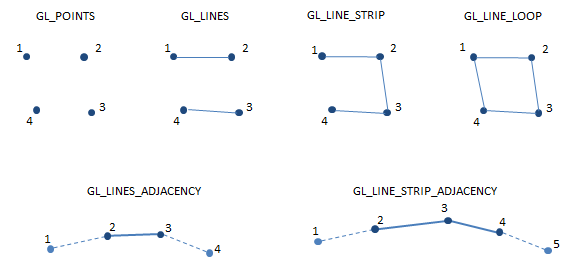
\includegraphics[scale=0.7]{02theorie/openglPrimitives.png}
	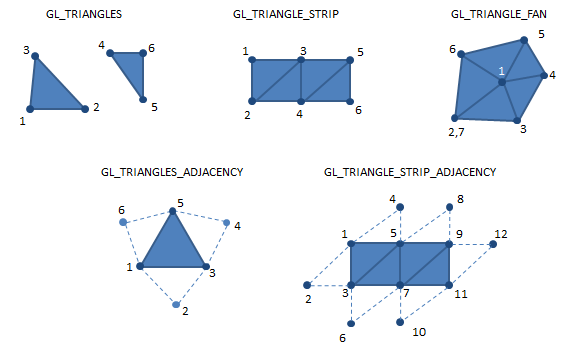
\includegraphics[scale=0.7]{02theorie/openglPrimitives2.png}
	
	
	Quelle: http://www.lighthouse3d.com/tutorials/glsl-tutorial/primitive-assembly/
	\caption{OpenGL Primitives}\label{OpenGLPrimitives}
\end{figure}


\begin{figure}
	\centering
	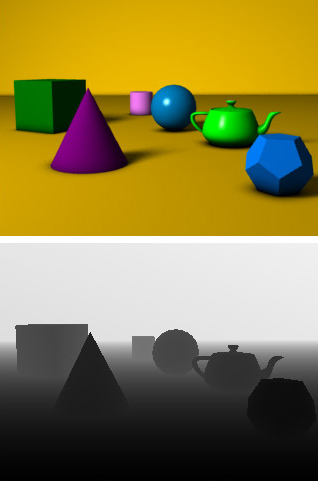
\includegraphics[scale=0.5]{02theorie/DepthBuffer.jpg}
	
	
	Oben: Color, Unten: Depth
	
	Quelle: https://de.wikipedia.org/wiki/Datei:Z-buffer\textunderscore no\textunderscore text.jpg
	\caption{Color- und Depth-Buffer}\label{DepthBuffer}
\end{figure}


\begin{figure}
	\centering
	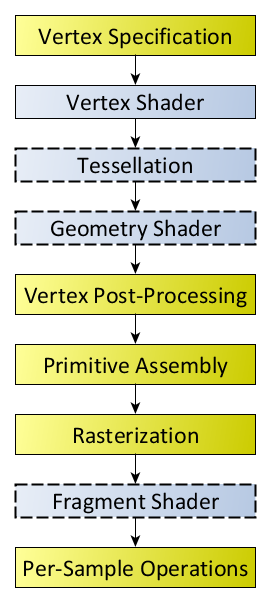
\includegraphics[scale=0.4]{02theorie/RenderingPipeline.png}
	
	
	Quelle: https://www.khronos.org/opengl/wiki/Rendering\textunderscore Pipeline\textunderscore Overview
	\caption{OpenGL Pipeline}\label{RenderingPipeling}
\end{figure}
\subsection{Physically Based Rendering}

In einer 3D-Szene eines Videospiels will man natürlich komplexere Objekte als Primitives darstellen. Diese Objekte bestehen aus vielen Primitives, wobei als Primitive Dreiecke genommen werden. Die Art der Zusammensetzung ist unterschiedlich, manchmal kann es von Vorteil sein aneinander hängende Dreiecke zu verwenden, aber meistens werden einfach einzelne Dreiecke gerendert. Einige Programme verwenden auch andere Polygone, aber diese bestehen auch nur aus Dreiecken, daher macht das keinen Unterschied. Ein Objekt, gebildet aus Dreiecken, nennt man \textit{Mesh}. Als Beispiel ist das Mesh eines Delfins in \cref{Dolphin} dargestellt. Die Farbe eines Objektes wird aus einem 2D Bild gelesen, genannt \textit{Textur}. Dafür besitzt jeder Vertex zusätzlich zu seiner Position eine 2D-Position auf der Textur, so kann ermittelt werden welche Pixel der Textur verwendet werden sollen. Mit Mesh und Textur ist es möglich ein Objekt in einer 3D-Szene anzuzeigen, aber es würde in einem Videospiel nicht überzeugen, da kommt \ac{PBR} ins Spiel. \ac{PBR} ist eine Möglichkeit eine realistischere 3D-Szene zu erzeugen in dem physikalische Phänomene wie Licht berücksichtigt werden. Wie ein Objekt auf Licht reagiert, hängt von verschiedenen Größen ab, wie die eigentliche Farbe des Objekts, die Oberflächenstruktur, aber auch die Farbe und Richtung des einfallenden Lichts. Alle Eigenschaften eines Objekts die sich auf die Farbe auswirken werden in einem \textit{Material} zusammengefasst. Ein zurenderndes  Objekt besitzt beides: ein Mesh und ein Material, was zusammengefasst \textit{Model} genannt wird.

Es gibt zwei Arten von Lichtquellen in der FM3D-Engine: \textit{Directional Light} und \textit{Point Lights}. Eins Directional Light besitzt, wie der Name sagt, eine Richtung aber keine Position. Es kann verwendet werden um zum Beispiel die Sonne darzustellen. Diese ist soweit von der Erde entfernt, dass die Position irrelevant ist, die Richtung dagegen ist wichtig und von der Tageszeit abhängig. Point Lights sind das genaue Gegenteil Sie besitzen keine Lichtrichtung sondern scheinen in alle Richtungen gleich, dafür besitzten sie aber eine genau festgelegte Position, welche wichtig ist, da die Lichtstärke mit zunehmendem Abstand kleiner wird. Point Lights können verwendet werden um die meisten Lichtquellen darzustellen wie Laternen oder Fackeln. Man kann aber nicht nur zwischen Lichtquellen unterscheiden sondern auch zwischen verschiedenen Arten des ausgesendeten Lichts. Die FM3D-Engine verwendet ein Lichtmodell genannt "Ambient/Diffuse/Specular". \textit{Ambient light} ist das Licht welches man jeden Tag sieht, auch wenn gerade keine Sonne scheint oder man sich nicht in direkter Nähe einer Lichtquelle befindet. Es entsteht dadurch, dass Licht von allen Objekten wieder teilweise reflektiert wird und so eine schwache und gleichmäßige Beleuchtung entsteht. Ohne diese wäre es hinter einem Haus, welches die Sonne verdeckt, komplett finster. Die zweite Lichtart ist \textit{Diffuse light}, welches abhängig von dem Auftrittswinkel des Lichtstrahls ist. Die dem Licht zugewandte Seite eines Würfels heller ist als die nur teilweise zugewandte Seite und die abgewandte Seite erfährt gar kein Diffuse light. \textit{Specular light} modelliert die Lichtstrahlen, welche von einem Objekt reflektiert und in die Linse der Kamera bzw. in die Augen des Betrachters gelangen. Dies wird als blendendes, helles Licht wahrgenommen und ist oft auf metallischen Obeflächen zu erkennen. Diese drei Lichtarten sind in \cref{Img:Lights} dargestellt.

Alle Lichtberechnungen müssen für jeden Pixel ausgeführt werden und laufen daher im Fragment shader ab.
Um die Farbe eines gerenderten Pixels zu bestimmen benötigen wir einige Informationen: Die Position des Pixels, die Farbe des Pixels, den Normalenvektor des Pixels und Specular factor des Pixels. Diese 4 Informationen reichen für alle Lichtberechnungen aus. Die Phase in der sie erstellt bzw. berechnet werden ist unterschiedlich. Ein Teil wird außerhalb des Programms in externen Programmen erstellt und als Vertex im Mesh oder als Information im Material. Dabei kann man unterscheiden zwischen: Information die sich zwischen verschiedenen Objekten unterscheidet aber nicht innerhalb des Objekts, Information die für jeden Vertex anders ist aber für jeden Pixel nur linear interpoliert werden muss und Information die für jeden Pixel anders ist. Ersteres ist das einfachste und kann einfach im Material gespeichert werden, da jedes Objekt ein eigenes Material haben kann und es anders als ein Mesh nicht viel Speicher benötigt. Die Vertexinformationen werden im \ac{VBO} des Mesh gespeichert und automatisch linear interpoliert wenn sie an den Fragment shader weiter gegeben werden. Pixelinformationen müssen einzeln in einer Textur gespeichert werden, diese ist dann im Material enthalten, wobei sie nur referenziert wird, damit verschiedene Materials die gleichen Texturen verwenden können. In den Vertexinformationen müssen hierfür zusätzlich Texturkoordinaten gespeichert werden. Daraus ergeben sich die folgenden Werte:

\begin{table}
	\caption{Vertex Aufbau}
	\label{table:VertexAufbau}
	\centering
	\begin{tabular}{lll}\toprule[1.5pt]
		Datentyp & Name & Beschreibung \\\midrule
		3D-Vektor & Position & Position des Vertex \\
		2D-Vektor & Textur Koordinate & Position des Vertex auf der Textur \\
		3D-Vektor & Normal & Normalenvektor zum Dreieck \\
		32-Bit Farbe & Color & Farbe des Vertex (optional, Standard ist weiß) \\
		3D-Vektor & Tangent & Tangentenvektor des Dreiecks. Benötigt wenn \\
		 & & Normal maps verwendet werden. Siehe \cref{section:Normalmapping}\\\bottomrule[1.5pt]
	\end{tabular}
\end{table}
\begin{table}
	\caption{Material Aufbau}
	\centering
	\begin{tabular}{lll}\toprule[1.5pt]
	Datentyp & Name & Beschreibung \\\midrule
	32-Bit Farbe & Color & Farbe des gesamten Objekts \\
	Textur & Color Texture & Gibt die Farbe jedes Pixels des Objektes an \\
	Textur & Normal map & Gibt den Normalenvektor jedes Pixels an. \\
	 & & Genaueres in \cref{section:Normalmapping} \\
	Float & Specular factor & Faktor für das resultierende Specular light \\
	Textur & Specular map & Specular factor für jeden Pixel. Der Faktor \\
	 & & des ganzen Objekts wird weiterhin verwendet \\
	 Boolean & UseWireframe & Gibt an ob ganze Dreiecke gerendert werden sollen\\
	  & & oder nur die Kanten. (Nützlich für Debugging)\\\bottomrule[1.5pt]
\end{tabular}
\end{table}


\begin{figure}
	\begin{center}
		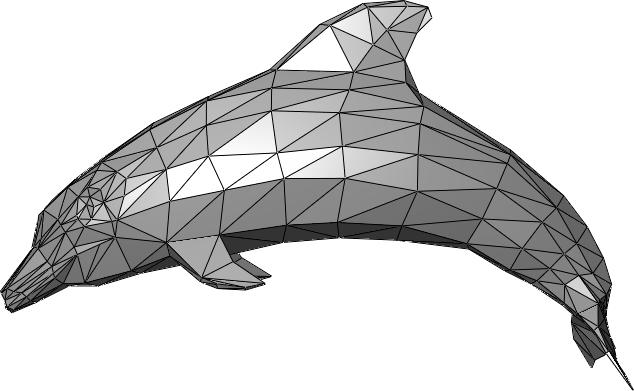
\includegraphics[width=0.5\textwidth]{06anhang/bilder/delphin.jpg}
		\caption{Mesh eines Delfins}
		\label{Dolphin}
	\end{center}
\end{figure}
\begin{figure}
	\centering
	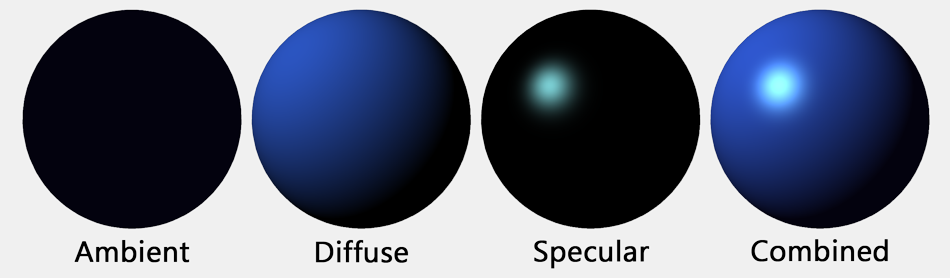
\includegraphics[scale=0.4]{02theorie/amb_diff_spec.png}
		
	Quelle: https://clara.io/img/pub/amb\textunderscore diff\textunderscore spec.png
	\caption{Lights}\label{Img:Lights}
\end{figure}
\subsection{Normalmapping}
\label{section:Normalmapping}

Um die visuelle Qualität eines Models zu erhöhen, so muss man das Modell genauer modellieren und somit resultieren mehr Dreiecke. 
Damit erhöht sich aber auch der Rechenaufwand für dieses Model und ab einer bestimmten Grenze ist die gewonnene Qualität nur sehr gering, der Rechenaufwand aber um so größer. Um ein Model trotzdem noch hochauflösender darzustellen wird ein Vorgang namens \textit{Normalmapping} verwendet. 
Dieser baut auf Lichtberechnungen auf, denn ohne Licht gibt es keine zu erkennende verbesserte Qualität. Normalerweise hat jeder Vertex einen Normalenvektor und für einen Pixel wird er zwischen den 3 Vertices interpoliert. Mit Normalmapping weißt man jedem Pixel einen eigenen Normalenvektor zu, so ist es möglich die Oberfläche so aussehen zu lassen, als würde sie rau mit kleinen Unebenheiten sein, ohne den Rechenaufwand von dem Rendern vieler Dreiecke eines Meshes zu belasten.
Den Unterschied Sieht man in \cref{img:Normalmapping}. Die Normalenvektoren werden in einer Textur gespeichert, sodass sie mit den normalen Texturen-Koordinaten verwendet werden können. Diese Textur wird im Material abgespeichert.

In einer Textur können drei Werte abgespeichert werden, Rot, Grün und Blau, jeweils mit einem Wert von 0 bis 1. Ein Normalenvektor hat aber drei Komponenten mit jeweils Werten von -1 bis 1, daher muss dieser erst berechnet werden:

$ \overrightarrow{N} = 
\begin{pmatrix}
x \\ y \\ z
\end{pmatrix}
 = 2 \cdot \overrightarrow{C} - 1 = 
 \begin{pmatrix}
 2 \cdot r - 1 \\ 2 \cdot g - 1 \\ 2 \cdot b - 1
 \end{pmatrix}$
 
Der Normalenvektor $\begin{pmatrix}
	0 \\ 0 \\ 1
\end{pmatrix}$ zeigt direkt weg von dem Model, daher sind Normalmaps auch immer sehr bläulich, denn der meiste Anteil des Normalenvektors liegt in der Z-Komponente. Eine Beispiel Normalmap ist in \cref{img:Normalmap} zu sehen. Man kann diesen Vektor aber nicht direkt verwenden, da er im \textit{Tangent space} definiert ist. Dies bedeutet dass er relativ zu dem zugehörigen Dreieck steht.
Man benötigt zudem einen Normalenvektor im \textit{Object space}, also relativ zu dem Model. 
Zur Umwandlung wird eine 3x3 Matrix benötigt, die aus drei verschiedenen Vektoren des Tangent-Space gebildet wird. 
Es können hierbei drei beliebige nicht linear abhängige Vektoren verwendet werden. Man bemerkt schnell, dass wenn alle drei orthogonal zueinander verlaufen, es simpler und effizienter ist die Matrix zu erstellen. 
Der erste Vektor wird bereits angegeben. Dieser beschreibt den Standardnormalenvektor jedes Vertex. Hinzu kommt noch ein Tangentenvektor jedes Vertex. Dieser befindet sich ebenfalls im \ac{VBO} des Meshes, wie in \cref{table:VertexAufbau} abgebildet ist. Der dritte Vektor ist der Bitangentenvektor
und kann mittels Kreuzprodukt aus diesen beiden berechnet werden. Es ist nötig alle drei Vektoren zu normalisieren, bevor die Matrix erstellt wird.

Gegeben ist der Normalenvektor $\overrightarrow{N}$ und der Tangentenvektor $\overrightarrow{T}$

Die normalisierten Vektoren: $\overrightarrow{N_{0}} = \dfrac{\overrightarrow{N}}{|\overrightarrow{N}|}$\qquad	$\overrightarrow{T_{0}} = \dfrac{\overrightarrow{T}}{|\overrightarrow{T}|}$

Der Bitangentenvektor: $\overrightarrow{B} = \overrightarrow{N_{0}} \times \overrightarrow{T_{0}}$\qquad	$\overrightarrow{B_{0}} = \dfrac{\overrightarrow{B}}{|\overrightarrow{B}|}$

Die Matrix sieht dann so aus: $M =  \begin{pmatrix}
T_{0x} & B_{0x} & N_{0x} \\
T_{0y} & B_{0y} & N_{0y} \\
T_{0z} & B_{0z} & N_{0z} \\
\end{pmatrix}$

Diese Matrix wird für erhöhte Leistung im Vertex shader erstellt und dann dem Fragment shader übergeben. In diesem muss dann nur der Normalenvektor aus der Normalmap geladen werden, dafür werden die gleichen Texturekoordinaten verwendet wie bei der Color texture, und mit dieser Matrix multipliziert werden.

\begin{figure}
	\begin{center}
		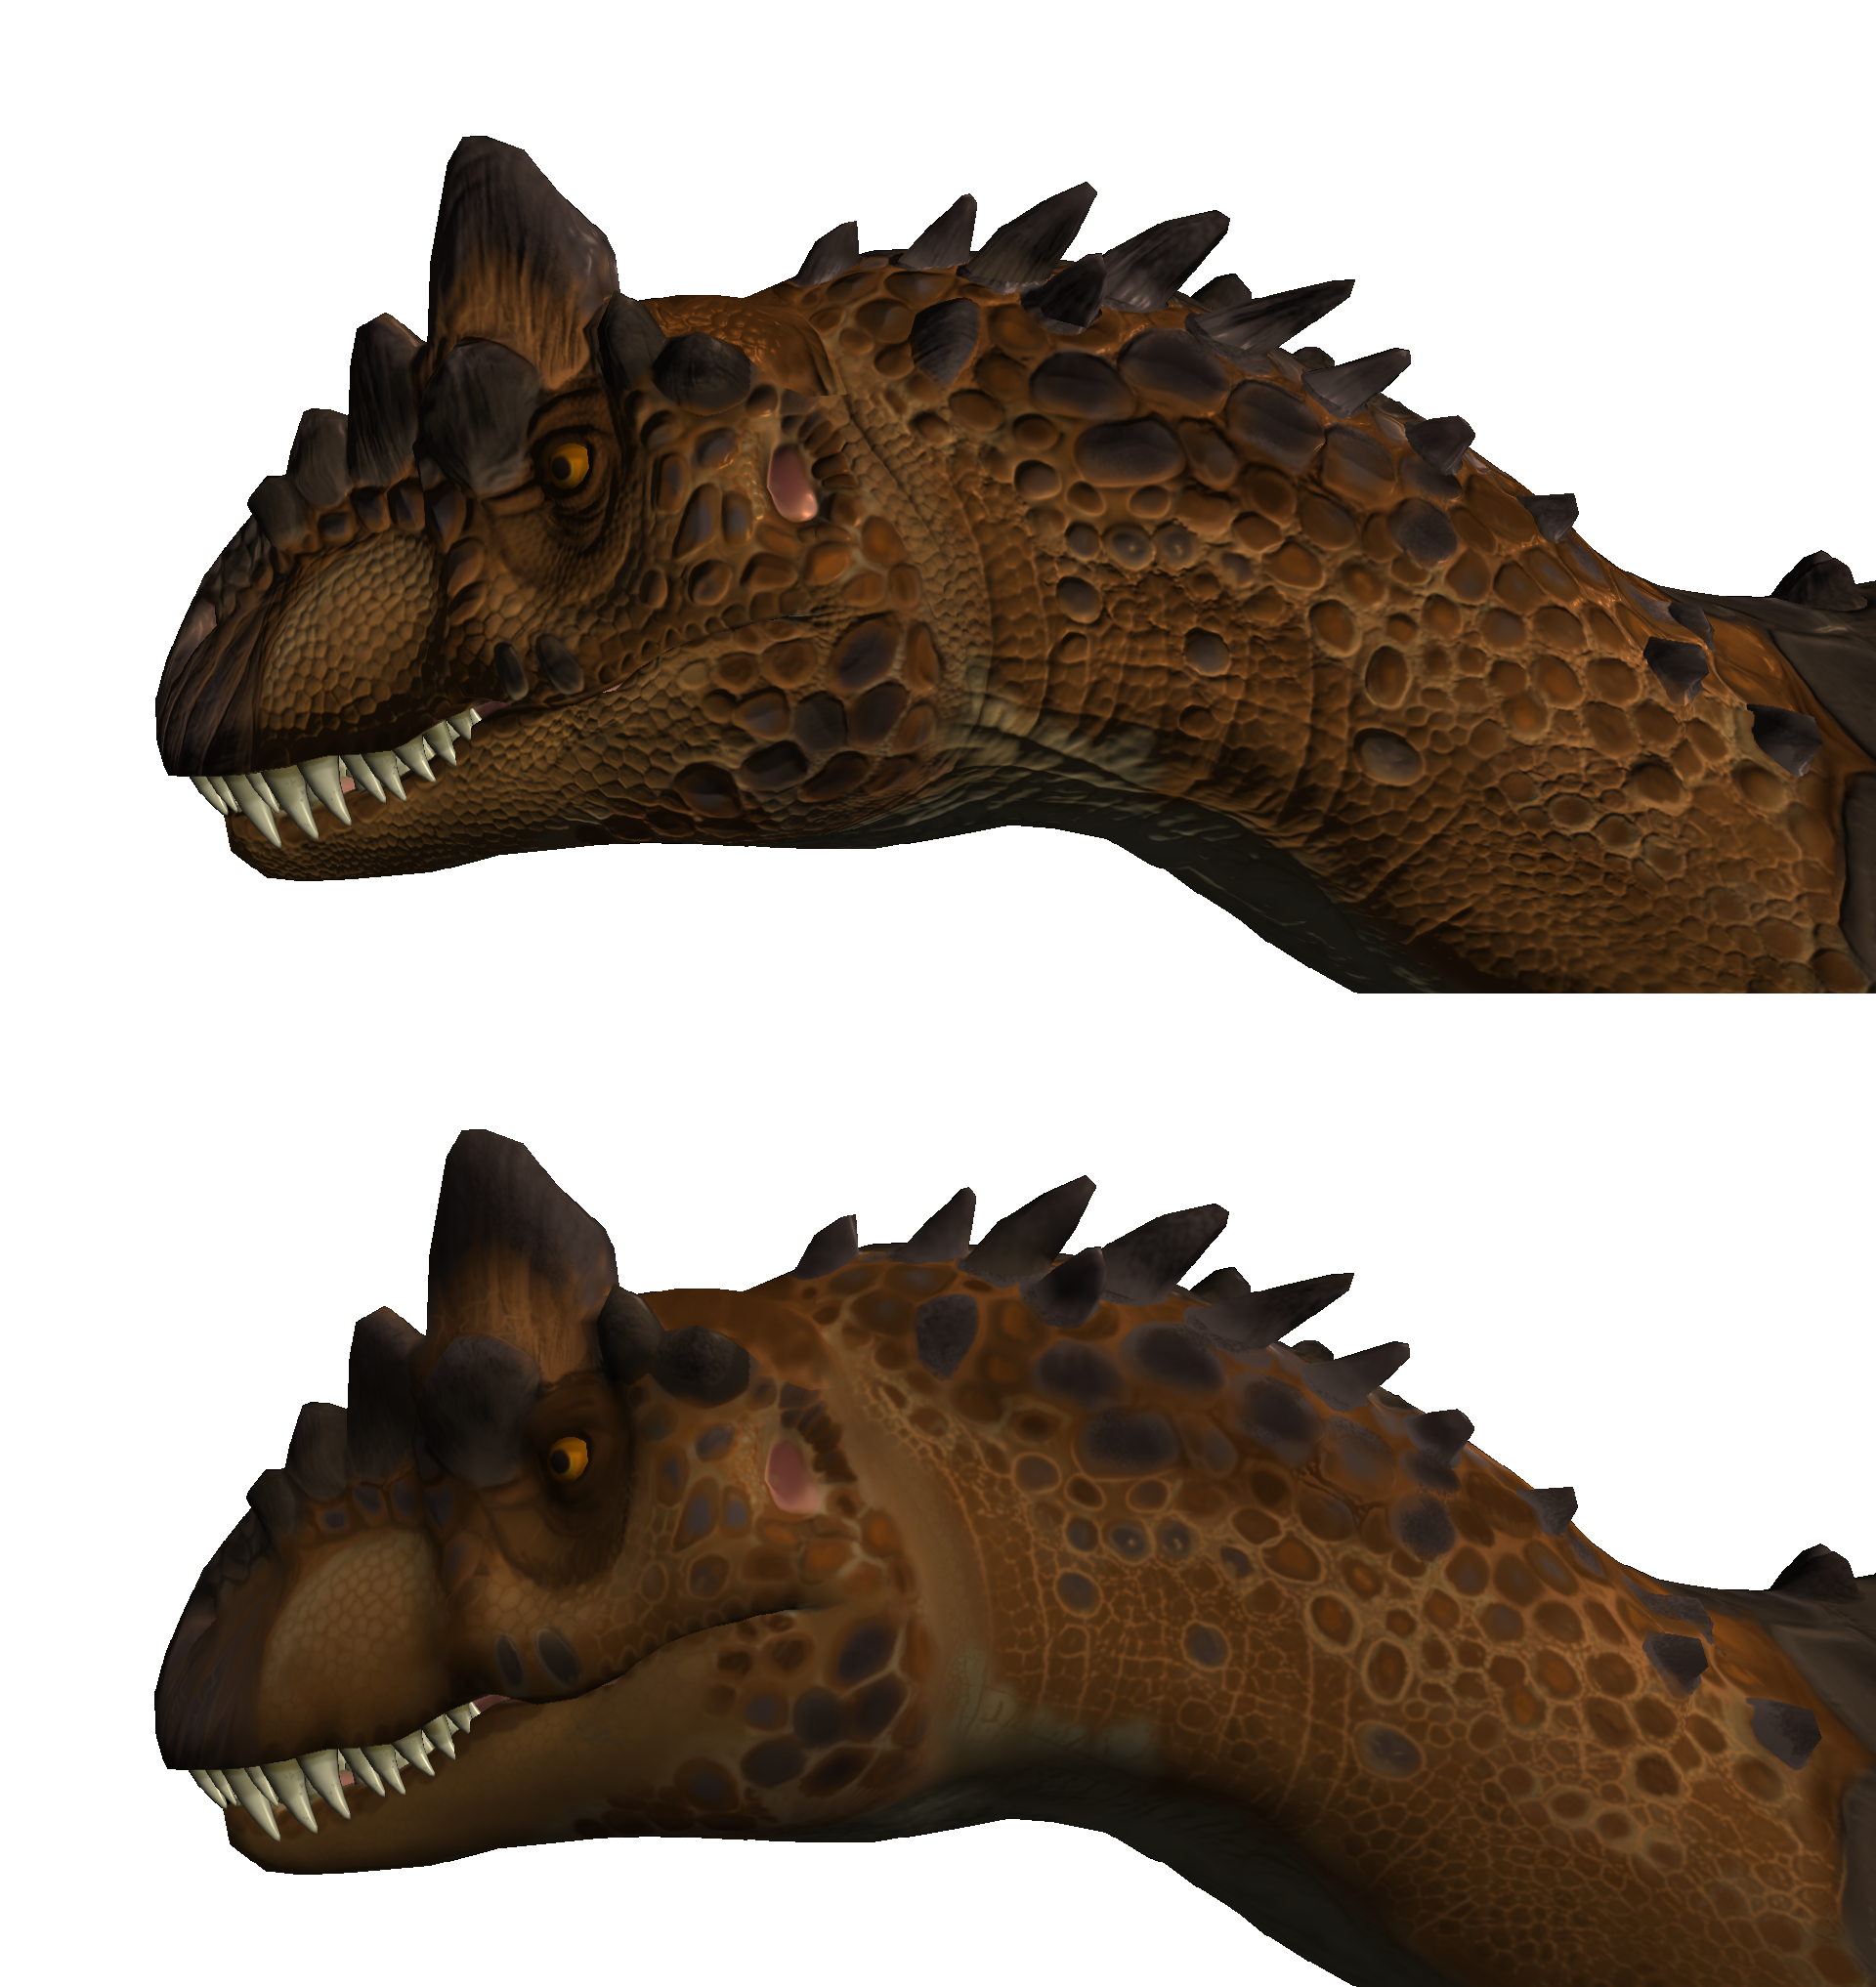
\includegraphics[width=0.5\textwidth]{02theorie/Normalmapping.png}
		
		Oben: mit Normalmapping, Unten: ohne Normalmapping
		
		Model: Allosaurus aus dem Spiel "`Ark: Survival Evolved"
		
		\caption{Normalmapping Beispiel}
		\label{img:Normalmapping}
	\end{center}
\end{figure}
\begin{figure}
	\begin{center}
		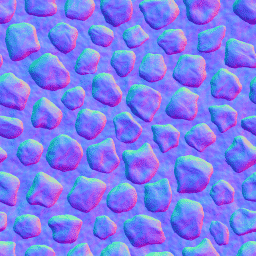
\includegraphics[width=0.4\textwidth]{02theorie/normalmap.png}
		
		Eine Beispiel Normalmap
		
		Quelle: http://www.bencloward.com/images/tutorial\textunderscore normals07.gif
		
		\caption{Normalmap Beispiel}
		\label{img:Normalmap}
	\end{center}
\end{figure}
\subsection{Animation}

Für einer lebendige Szene in einem Spiel reicht es nicht aus nur statische Models zu verschieben und zu drehen. Wenn man zum Beispiel ein Pferdmodel im Spiel einbindet und es nur nach vorne bewegt, wenn es laufen soll, so wirkt das Pferd nicht lebendig und es sähe so aus als würde man eine Statue verschieben. Man muss in diesem Falle also ein Modell animieren.
Die FM3D-Engine verwendet eine Animationsart namens \textit{Skeletal-Animation}. Hierbei bekommt jedes animierte Mesh ein Skelett zugewiesen, wobei sich mehrere verschiedene Meshes das gleiche Skelett teilen können. Zum Beispiel könnte es in einem Spiel ein Mesh für einen Ritter und eines für einen Bauern geben. Diese sehen unterschiedlich aus, aber beide könnten das gleiche Skelett haben und somit die gleichen Animationen.

Ein Skelett besteht aus mehreren Knochen, die jeweils weitere Knochen besitzen. Wenn sich ein Knochen bewegt, bewegt er alle an ihm hängende Knochen und die wiederum alle an ihnen hängenden. 
Dies hat den Vorteilm, dass wenn sich der Knochen des linken Armes bewegt, sich auch gleichzeitig alle Fingerknochen bewegen würden. Jeder Knochen besitzt unabhängig von den anderen eine Ausgangsposition und eine ID.
Die Id wird verwendet um herauszufinden, welcher Knochen sich auf welchen Vertex auswirkt und welche Knochen gar nicht verwendet werden. Jeder Vertex kann von bis zu 4 Knochen transformiert werden. Dazu besitzt jeder Vertex 4 Knochen-IDs und 4 floats die angeben wie stark sich ein Knochen auf den Vertex auswirkt, wie in \cref{table:VertexAufbau} zu sehen ist. Diese Daten werden in einem externen Programm beim Erstellen des Meshes festgelegt. Dieser Vorgang wird \textit{Weight painting} genannt, da die Zuweisung durch eine Art Malen in den Modellierungsprogrammen geschieht. Ein Beispiel aus dem Programm Blender ist in \cref{Img:Skeleton} zu sehen.

Eine Animation besitzt zu verschiedenen Zeitpunkten eine Position, Rotation und Skalierung für einen Knochen genannt \textit{Keyframe}. Dabei ist es nicht nötig, dass alle Knochen die gleiche Anzahl an Keyframes haben oder einen Keyframe an der gleichen Zeitposition. Es ist auch möglich, dass Keyframes nicht Position, Rotation und Skalierung auf einmal beinhalten sondern nur eins oder zwei davon. Um den Zustand aller Knochen zu einem bestimmten Zeitpunkt herauszufinden fängt man am obersten Knochen der Hierarchie an und arbeitet sich dann schrittweise nach unten, da die unteren Knochen von den oberen abhängig sind. 
Falls der Zustand zu diesem Zeitpunkt nicht zufällig durch die Keyframes genau definiert ist, muss zwischen den zwei am nächsten liegenden Keyframes interpoliert werden.

Für die Position und Skalierung kann zwischen den Keyframes linear interpoliert werden:

$t_{0} \leq t \leq t_{1}$ \qquad $t_{0} < t_{1}$ \qquad Keyframes: $\overrightarrow{P_{0}}, \overrightarrow{P_{1}}$

$f = \dfrac{t - t_{0}}{t_{1} - t_{0}}$

$\overrightarrow{P} = ((\overrightarrow{P_{0}} \cdot (1 - f)) + (\overrightarrow{P_{1}} \cdot f)$

Für die Rotation muss \ac{SLERP}\cite{WikiSlerp} angewendet werden, dadurch bleibt die Kreisgeschwindigkeit über die Zeit konstant. Die Berechnung erfolgt für zwei Quaternionen, die eine Rotation repräsentieren.

$t_{0} \leq t \leq t_{1}$ \qquad $t_{0} < t_{1}$ \qquad Keyframes: $Q_{0}, Q_{1}$

$f = \dfrac{t - t_{0}}{t_{1} - t_{0}}$

$\phi = Q_{0} \cdot Q_{1}$

$\theta = \arccos(\phi) \cdot f$

$Q_{2} = Q_{1} - Q_{0} \cdot \phi$

$Q = Q_{0} \cdot \cos(\theta) + Q_{2} \cdot \sin(\theta)$

\begin{figure}
	\centering
	\begin{minipage}{0.49\textwidth}
		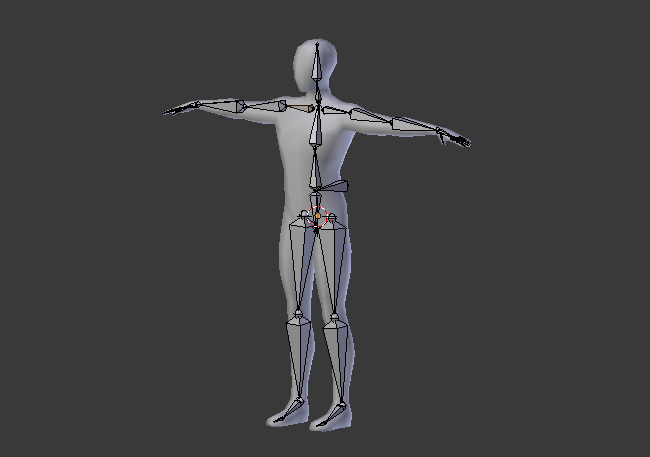
\includegraphics[width=\textwidth]{02theorie/skeleton.jpg}
	\end{minipage}
	\hfill
	\begin{minipage}{0.49\textwidth}
		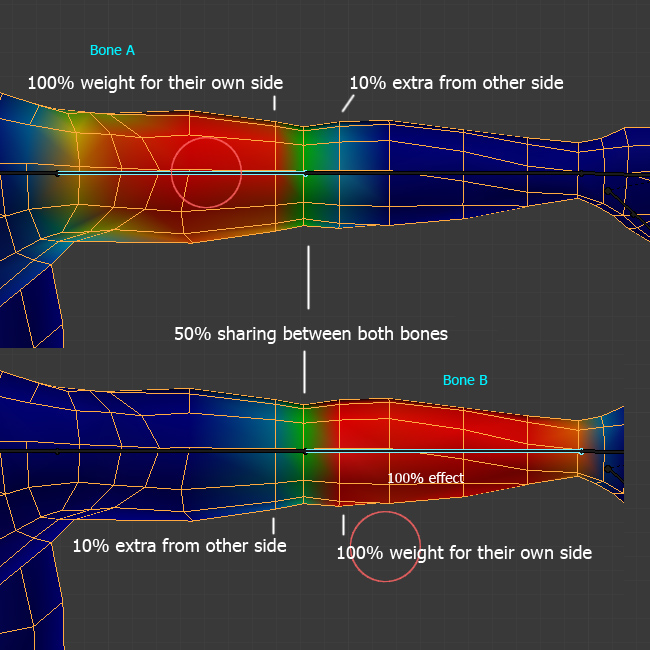
\includegraphics[width=\textwidth]{02theorie/weightpainting.jpg}
	\end{minipage}

	
	Links: Skelett in Blender, Rechts: Weight painting eines Arms in Blender 
	
	Quelle: https://cgi.tutsplus.com/tutorials/building-a-basic-low-poly-character-rig-in-blender--cg-16955
	\caption{Blender Skelett}\label{Img:Skeleton}
\end{figure}